\appendix
\chapter{Identidad visual de los algoritmos}

Las figuras comparativas de este documento emplean una codificación visual consistente: cada algoritmo mantiene el mismo color y el mismo marcador en todas las representaciones, de modo que el lector pueda seguir un competidor concreto a través de las distintas figuras sin recurrir a la leyenda en cada caso.

\begin{figure}[H]
\centering
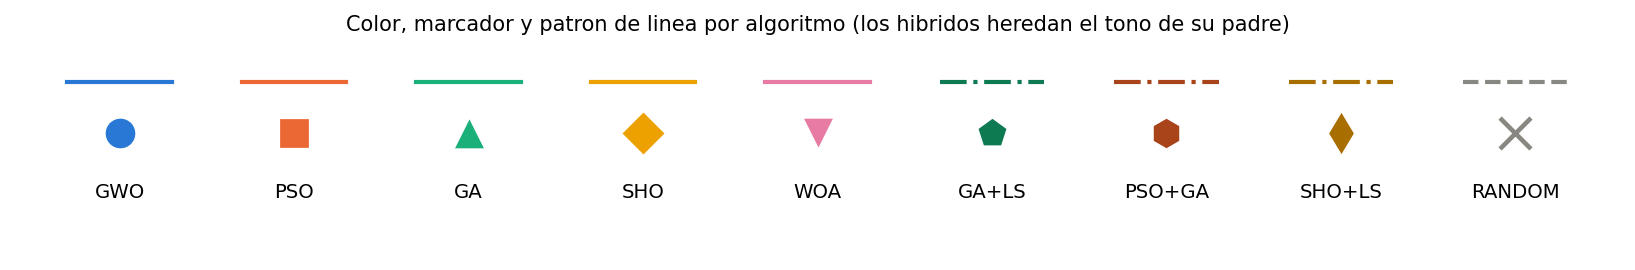
\includegraphics[width=0.82\textwidth]{figures/fig04_identidad_visual.png}
\caption{Correspondencia entre algoritmo, color y marcador empleada de forma consistente en todas las figuras comparativas.}
\label{fig:identidad_visual}
\end{figure}

La forma del marcador actúa como codificación primaria y el color como refuerzo secundario. Esta redundancia evita que la identificación de nueve series dependa exclusivamente de la percepción cromática y mantiene la lectura al imprimir en escala de grises. Los tres híbridos heredan el tono de su padre y se distinguen por un patrón de línea de puntos y rayas y por un marcador propio.

\chapter{Plan de trabajo del proyecto}

El trabajo recogido en esta tesis corresponde a la ejecución completa del primer paquete de trabajo de un proyecto de investigación de mayor alcance, cuya estructura se documenta aquí para situar el aporte realizado.

\section{WP1: Evaluación de metaheurísticas para HRES-H$_2$}

Su propósito es evaluar la aplicabilidad, flexibilidad y limitaciones de las metaheurísticas de población aplicadas a configuraciones HRES-H$_2$, identificando las características críticas del problema y las limitaciones de los enfoques existentes.

\begin{itemize}
    \item \textbf{Tarea 1.1:} revisión del estado del arte sobre modelos HRES-H$_2$ y análisis de su complejidad computacional. \textit{Completada}, véase el marco teórico.
    \item \textbf{Tarea 1.2:} revisión del estado del arte sobre metaheurísticas modernas basadas en población. \textit{Completada}, con la incorporación de GWO \cite{Mirjalili2014GWO}, PSO \cite{Kennedy1995PSO}, GA \cite{Goldberg1989GA}, SHO \cite{Dhiman2017SHO} y WOA \cite{Mirjalili2016WOA}.
    \item \textbf{Tarea 1.3:} análisis de enfoques híbridos de optimización basados en población. \textit{Completada}, con la taxonomía de Talbi \cite{Talbi2002Taxonomy} y tres híbridos integrativos de bajo nivel: GA+LS \cite{Moscato1989Memetic}, PSO+GA \cite{Kao2008HybridGAPSO} y SHO+LS. La integración de componentes de aprendizaje se traslada al WP2.
    \item \textbf{Tarea 1.4:} implementación, experimentación y evaluación de los enfoques seleccionados. \textit{Completada} para las cuatro instancias y las sensibilidades declaradas; véanse los capítulos de diseño experimental y de resultados.
\end{itemize}

\section{WP2: Integración de componentes de aprendizaje basados en ANN}

Orientado al diseño e integración de redes neuronales artificiales dentro de marcos de optimización híbrida, con el objetivo de reducir el número de evaluaciones costosas mediante modelos sustitutos de la función objetivo. Su pertinencia queda reforzada por los resultados de esta tesis: siendo la simulación horaria el costo dominante, un modelo sustituto suficientemente preciso permitiría ampliar el presupuesto efectivo de búsqueda en órdenes de magnitud.

\section{WP3: Extensión ambiental y multiobjetivo}

Aborda la incorporación de métricas de sostenibilidad al proceso de optimización, complementando los criterios técnicos y económicos con indicadores ambientales bajo una formulación multiobjetivo de frente de Pareto.

\section{WP4: Difusión y comunicación de resultados}

Contempla la comunicación de los avances metodológicos y de los resultados obtenidos a audiencias académicas y técnicas.

\chapter{Reproducibilidad del experimento}

\section{Artefactos computacionales}

La totalidad de los resultados reportados en esta tesis se regenera a partir de los siguientes artefactos:

\begin{itemize}
    \item \texttt{notebooks/H2\_HRES\_trabajo.ipynb} --- cuaderno autocontenido de 22 secciones que incluye configuración, modelos físicos y económicos, pruebas deterministas, reproducción parcial, las cuatro instancias y su óptimo exacto por fuerza bruta, seis optimizadores clásicos y tres híbridos, análisis estadístico y sensibilidades.
    \item \texttt{notebooks/src/hourly\_2008.csv} --- serie meteorológica de 8.784 registros obtenida de NASA POWER \cite{NasaPower}; el caso principal excluye las 24 horas del 29 de febrero.
    \item \texttt{notebooks/src/data\_provenance.csv} --- procedencia disponible del archivo horario y declaración explícita de que la versión de API no quedó registrada.
    \item \texttt{scripts/execute\_notebook.py} --- ejecutor reproducible de los modos rápido y completo.
    \item \texttt{notebooks/results/} --- tablas CSV de validación, instancias, fuerza bruta, corridas, historiales, semillas, estadística y sensibilidades exportadas por el cuaderno, con una columna \texttt{instance} donde corresponde.
    \item \texttt{notebooks/cache/} --- resultados reducidos de la fuerza bruta por instancia (mejor $W$ por catálogo, envolvente y celdas de control), indexados por una huella del escenario, de los datos y del paso. No se versiona; se regenera.
    \item \texttt{scripts/generar\_tablas\_latex.py} y \texttt{scripts/extraer\_figuras.py} --- generación automática de tablas y figuras para el documento.
\end{itemize}

\section{Requisitos y ejecución}

El cuaderno requiere Python 3.13, \texttt{numpy}, \texttt{pandas}, \texttt{matplotlib}, \texttt{scipy}, \texttt{nbformat} y \texttt{nbclient}. No requiere conexión de red en tiempo de ejecución ni la instalación de paquetes propios del proyecto.

La ejecución se controla mediante el argumento \texttt{--mode} del script o el interruptor equivalente situado en la primera celda de código:

\begin{itemize}
    \item \texttt{MODO = "rapido"} --- 3 semillas, 8 individuos y 8 iteraciones, con fuerza bruta a paso de 1 MW. Unos diez minutos de ejecución. Destinado a verificar que el cuaderno se ejecuta de principio a fin sin errores.
    \item \texttt{MODO = "completo"} --- \Replicates{} semillas, \Population{} individuos y \Iterations{} iteraciones: \RequestsPerInstance{} solicitudes de evaluación de diseños anuales por instancia, \TotalDesignRequests{} en total, más \BruteForceDesignsTotal{} diseños de fuerza bruta (unas \BruteForceElapsedHours{} horas). El tiempo depende del equipo empleado. Es el modo con el que se generaron las cifras y figuras de este documento.
\end{itemize}

\section{Determinismo}

Cada corrida se inicializa con un generador de números pseudoaleatorios propio, derivado de una semilla explícita del conjunto $\{42, 43, \ldots, 71\}$. La reproducibilidad no depende por tanto del estado global del intérprete ni del orden de ejecución de las celdas. Dos ejecuciones del cuaderno en modo completo producen resultados numéricamente idénticos.

\section{Extracción de las figuras}

Las once figuras incluidas en este documento se extraen directamente de las salidas persistidas en el cuaderno ejecutado mediante el script \texttt{scripts/extraer\_figuras.py}. Cada celda que produce una figura lleva un marcador \texttt{\# FIG: nombre} en su código, de modo que la correspondencia no depende de la posición de la celda y las imágenes corresponden exactamente a la misma ejecución de la que provienen las cifras citadas en el texto.

\chapter{Contrastes completos por instancia}

El análisis principal usa la familia planificada de 12 contrastes por instancia. Para completitud se reportan aquí los 36 pares de cada instancia, con Mann--Whitney bilateral, corrección de Holm sobre los 36 pares y $A_{12}$ con intervalo bootstrap al 95\,\%, junto con las matrices de $A_{12}$.

\begin{figure}[H]
\centering
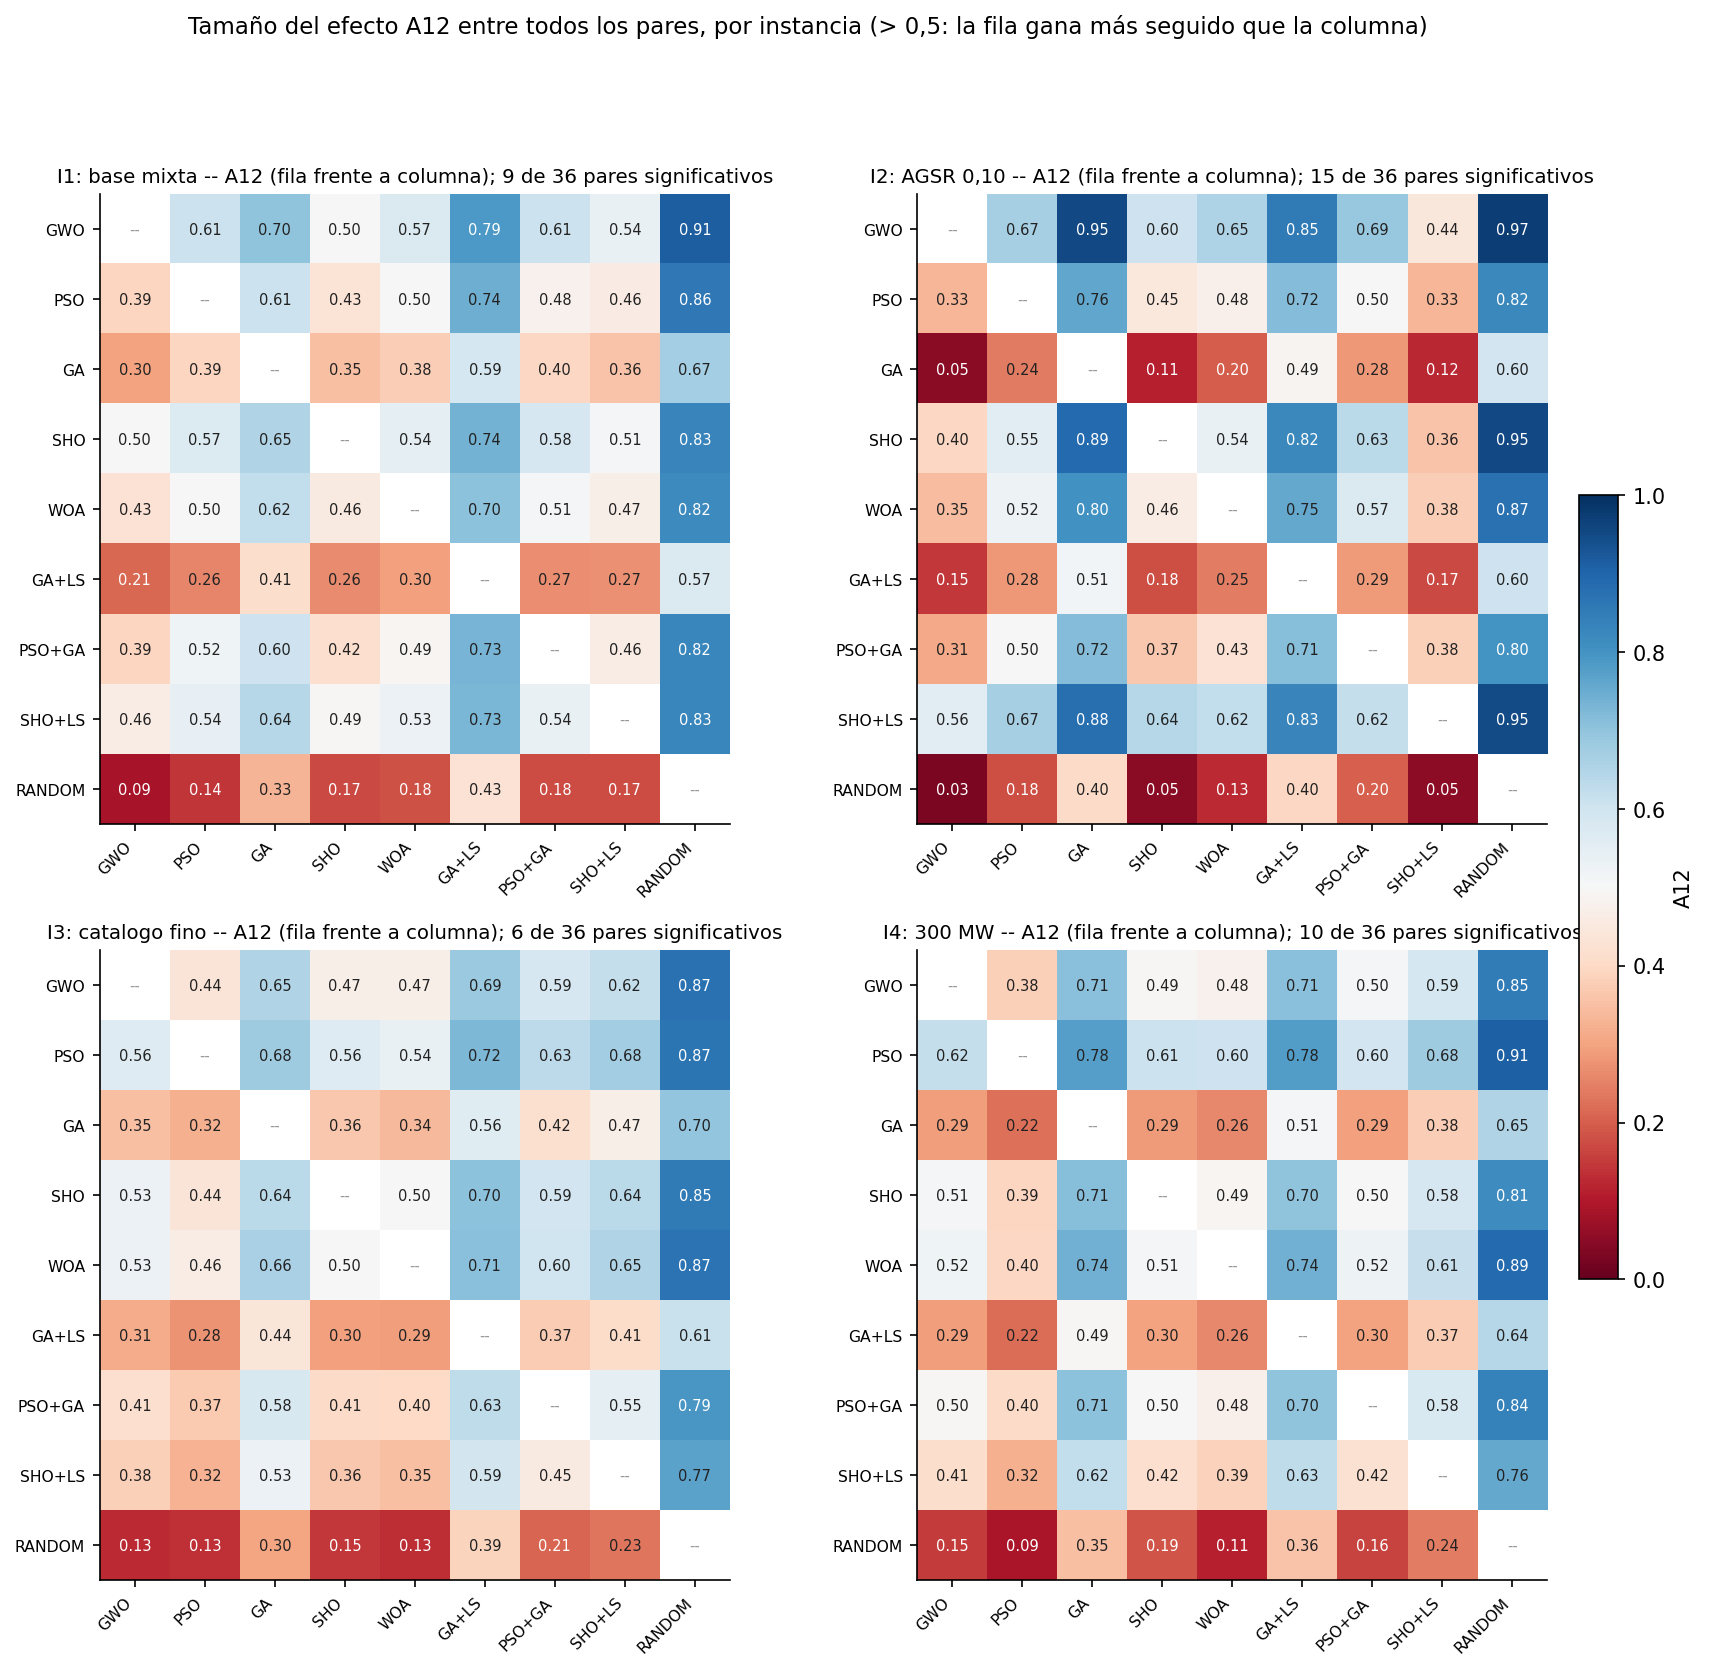
\includegraphics[width=0.98\textwidth]{figures/fig11_matrices_a12.png}
\caption{Tamaño del efecto $A_{12}$ entre todos los pares de algoritmos, por instancia. Valores mayores que 0,5 indican que la fila obtiene menor LCOE con más frecuencia que la columna.}
\label{fig:matrices_a12}
\end{figure}

\TablaParesCompletaAutoA
\TablaParesCompletaAutoB
\TablaParesCompletaAutoC
\TablaParesCompletaAutoD
